\chapter{Prior contribution and limits of the explanation}
\label{ch:analysis}

The forecasting comparisons establish where VolPFN is useful, but leave the explanation of its advantage open. We investigate that explanation in stages: matching two simulation designs, changing training loss and output, and strengthening the historical comparator. We then ask whether a small rule retains useful prediction and whether the network tracks simulated volatility nearly as well as a privileged reference. Each comparison tests a different part of the proposed explanation.

\section{A matched test of the prior package}
\label{sec:matched-prior}

To test the prior's contribution, we train network pairs on different simulated histories while matching the remaining settings. Matching initial weights and training allocation reduces variation from initialisation, duration and checkpoint selection. The intended intervention is the simulation design, which allows a more specific interpretation than a comparison between unrelated forecasting systems.

\subsection{Why this alternative, and what changes?}

The broad design samples seven volatility families (Table~\ref{tab:simulation-prior}). Its Mat\'ern alternative draws a hidden log-variance path from a Gaussian-process covariance model \citep{rasmussen2006gaussian}, varying irregularity and persistence without a return-driven scale recursion. Applied to the turbulent-week illustration, these designs provide different explanations of similar observed returns.

For Mat\'ern histories, we sample equally from nine combinations of smoothness values 0.1, 0.5 and 1.5 and length scales 30, 120 and 500 observations. Log-variance standard deviation is uniform between 0.3 and 1.5. These are specified settings rather than literature-prescribed optima. Both experimental \emph{arms} retain the same innovation generator and probabilities of jumps, serial correlation, drift and stale observations. The comparison changes latent-volatility design while sharing these disturbances. Overlapping diagnostic ranges do not make all observable features identically distributed, and this construction represents one alternative rather than every generic prior.

All five pairs retain the \emph{fixed-final} checkpoint at update 20,000 without validation-based selection. Architecture, normalisation, losses, optimisation and allocation agree within pairs, although their random histories may differ. The intervention therefore concerns the combined design under a finite recorded training procedure, not an idealised fully converged predictor (Appendix~\ref{app:closure_protocol}).

\subsection{The target and decision rule}

Acquisition and quality gates define the population before scoring. Both models then forecast the same roughly 22,500 returns across twenty indices in March 2022--August 2026. Eight candidates fail the rules rather than being excluded because of forecast gains. Prior contact with these histories remains documented in Section~\ref{sec:exposure}.

We compare scale by converting each predicted second moment to the zero-centred Student law with eight degrees of freedom defined in Chapter~\ref{ch:data}. The common-$t_8$ law holds scoring tails fixed, while the mixture output still affects the second moment being converted. No fitted multiplier can absorb differences in forecast level. We average scores across dates within markets, then give markets and seeds equal weight, so longer histories do not receive greater panel weight.

The decision rule considers uncertainty, the chosen effect-size threshold and market breadth. Section~\ref{sec:inference} specifies the tests, a mean of at least 0.005 nats per return and positive means in at least fifteen markets. The reserved broad-versus-GARCH slot stays in the multiplicity family despite being unrun. Equivalence uses its separate $\pm0.003$-nat margin. These requirements are unchanged from the specified decision rule.

\subsection{Results and their magnitude}

\begin{table}[!htbp]
\centering\small
\caption[Five matched prior pairs]{Broad-minus-Mat\'ern common-$t_8$ log-score gain, in nats per return. Each row pairs models with matching initialisation and training settings. All rows use the same locked 20-market sample.}
\label{tab:matched-prior-seeds}
\begin{tabular}{lr}
\toprule
Seed pair & Gain \\
\midrule
8101 & 0.005942 \\
8102 & 0.005217 \\
8103 & 0.004745 \\
8104 & 0.004335 \\
8105 & 0.005661 \\
\midrule
Equal-seed mean & 0.005180 \\
95\% conditional interval & $[0.001862,0.008151]$ \\
Holm-adjusted $p$ & 0.003199 \\
Positive markets & 17/20 \\
\bottomrule
\end{tabular}
\end{table}

The broad-minus-Mat\'ern common-$t_8$ gain averages about 0.0052 nats per return (Table~\ref{tab:matched-prior-seeds}). All five paired means and seventeen of twenty market means are positive. The conditional interval excludes zero, the adjusted test passes and the mean clears the size threshold. The experiment therefore meets all three requirements: support, magnitude and breadth.

Exponentiating the mean difference gives roughly half a percent higher density at observed returns on a geometric-average basis. This is a modest forecasting improvement rather than an investment return. The aggregate only narrowly clears 0.005, two pair means fall below that threshold, and a positive interval does not show that the population gain exceeds it. The equivalence interval also falls outside the declared band; Appendix~\ref{sec:prior-interpretation-details} retains its exact endpoints.

\begin{figure}[!htbp]
\centering
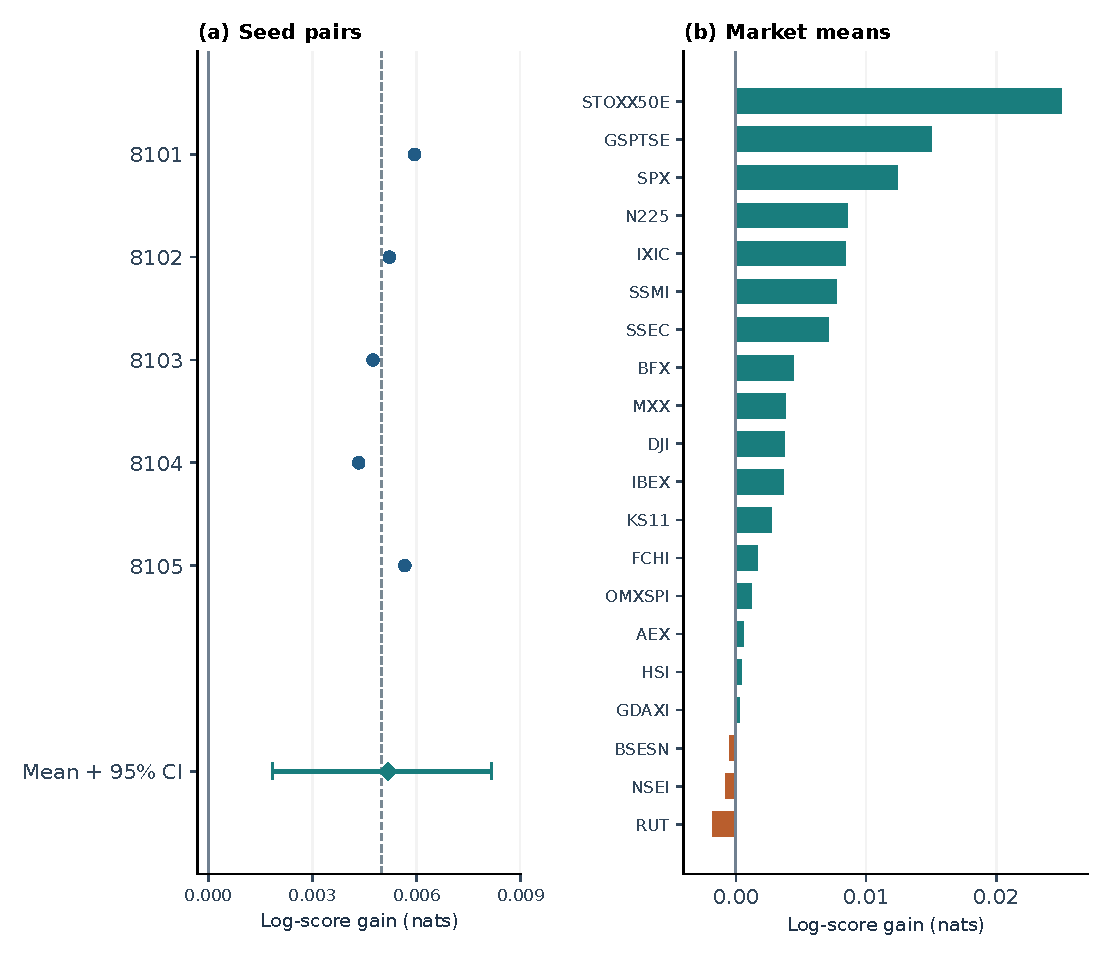
\includegraphics[width=\textwidth]{matched_prior.pdf}
\caption[Prior substitution by seed and market]{The broad-minus-Mat\'ern common-$t_8$ gain. Left: all five paired means and the aggregate conditional 95\% interval; the dashed line is the point-materiality gate, not a confidence bound. Right: the twenty equal-seed market means, with three negative values retained. Market and seed dots are descriptive, not separately tested effects.}
\label{fig:matched-prior}
\end{figure}

We next assess how concentrated the aggregate gain is by omitting market summaries from descriptive averages. STOXX50E, GSPTSE and SPX contribute about half of the net gain (Figure~\ref{fig:matched-prior}), so we examine their individual and joint omissions. These post-result calculations neither redefine the registered population nor create another confirmatory test.

\begin{figure}[!htbp]
\centering
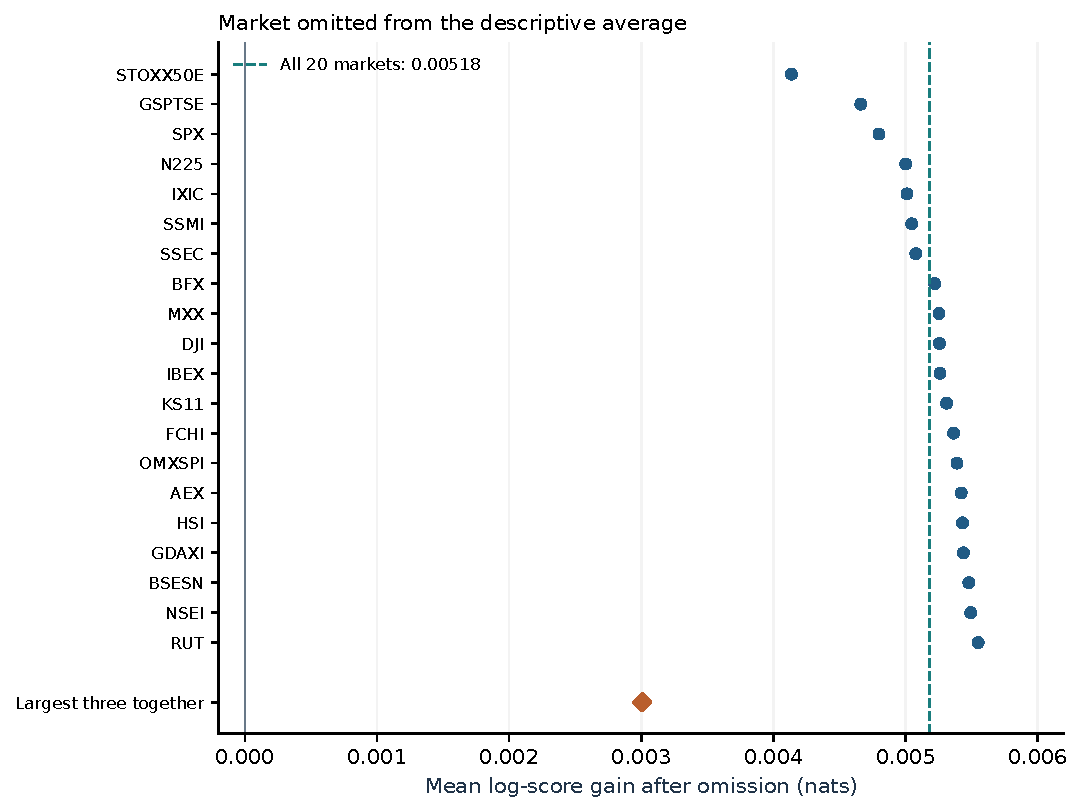
\includegraphics[width=\textwidth]{prior_market_influence.pdf}
\caption[Descriptive influence of individual markets]{Sensitivity of the broad-minus-Mat\'ern mean gain to omitting market summaries. Each single-omission point averages the remaining nineteen markets. The separate three-market omission excludes STOXX50E, GSPTSE and SPX, the largest observed positive contributors. These are post-result descriptive calculations on existing scores, with no new confidence intervals or registered hypothesis tests. The original twenty-market decision is unchanged.}
\label{fig:prior-market-influence}
\end{figure}

Every single-market omission leaves a positive mean of roughly 0.004--0.006 nats per return. Removing the three largest contributors together leaves about 0.003 across seventeen markets (Figure~\ref{fig:prior-market-influence}). The direction does not depend on one market, although the size depends on panel composition. Without additional intervals, these descriptive summaries establish no separate population effect.

The result supports the combined simulation design relative to this Mat\'ern alternative. Because several properties change together, it does not isolate return feedback, asymmetry or regime switching as the cause. Uncertainty also conditions on the ten fitted networks. A narrower matched intervention would be needed to identify one mechanism. We now turn to the completed changes in supervision, output and training source.

\section{What the component interventions establish}
\label{sec:new-components}

The component programme retains the supplied update budget while changing stated configurations. Its twenty runs compare auxiliary volatility supervision, distribution versus direct risk prediction, and synthetic versus historical windows on the 2015--February 2022 panel (Table~\ref{tab:new-components}). The results apply to these tested configurations rather than every implementation of each component.

\begin{table}[!htbp]\centering
\begingroup\small\setlength{\tabcolsep}{4pt}
\caption[Matched training-component interventions]{Component interventions, 2015--February 2022. Gain is comparator minus named reference squared-return QLIKE; positive favours the reference. All five seeds and 28 markets remain. Ordinary intervals and Holm probabilities use the separate three-slot family, 20,000 draws and 60-date blocks.}\label{tab:new-components}
\begin{tabular}{@{}>{\raggedright\arraybackslash}p{4.1cm}rcr@{}}
\toprule
Comparison & Gain & Ordinary 95\% interval & Holm $p$ \\
\midrule
Full versus noaux & -0.000581 & $[-0.001499,0.000321]$ & 0.206540 \\
Density noaux versus direct & 0.009540 & $[0.004052,0.015214]$ & 0.001300 \\
Synthetic versus historical noaux & 220.701975 & $[168.500456,263.777505]$ & 0.000150 \\
\bottomrule
\end{tabular}\endgroup\end{table}


Removing the simulated-volatility loss produces \emph{noaux}, while \emph{full} retains it. We detect no deterioration from removal: full's estimated gain is slightly negative and its interval crosses zero. Two seeds favour full and three favour noaux. Keeping the unused noaux head preserves initialisation matching. Its continued presence does not supply volatility supervision because that loss has been removed. This result concerns the tested supervision weight and budget; it establishes neither equivalence nor the absence of a useful alternative setting.

The noaux distribution configuration improves QLIKE over direct expected-squared-return prediction by about 0.010, with a positive interval and passing adjusted test. Matching the initial trunk and supplied synthetic batches controls those settings, but output and loss still change together. The evidence therefore supports the combination of output and loss. Direct has no native return distribution, and conversion to common-$t_8$ scoring does not create a learned density.

\begin{figure}[!htbp]\centering
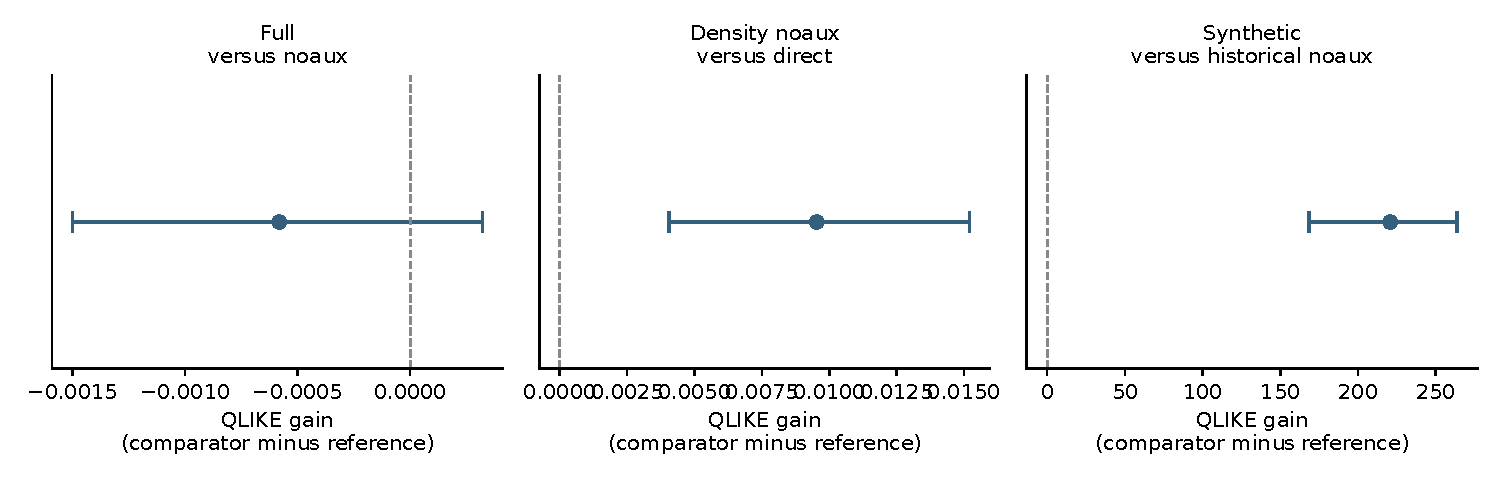
\includegraphics[width=\textwidth]{new_component_gains.pdf}
\caption[The three component interventions]{Comparator-minus-reference QLIKE gains and ordinary conditional 95\% intervals for the three registered component comparisons. Each panel has its own numerical axis because the historical failure is much larger. The intervals are not simultaneous; the separate three-slot Holm family supplies the adjusted tests.}
\label{fig:new-components}
\end{figure}

The original fixed-final historical model severely underpredicts some later risks. Mean QLIKE is about 221 versus 0.59 for synthetic noaux, despite a historical median near 0.55. More than fifteen thousand seed-level forecasts exceed QLIKE 100. This difference between mean and median shows why a typical-observation summary would hide the failures. Appendix~\ref{sec:prior-interpretation-details} retains exact counts.

The recorded checks of targets, scaling, alignment and the evaluation path found no clear defect. Historical training repeats about 70,000 distinct observations; low late-training likelihood loss alongside poor later calibration is consistent with memorisation or density collapse. These diagnostics do not identify a sole cause. The failure concerns that optimisation and selection procedure; it does not establish general inferiority of historical training. To assess how much the source comparison depends on this failure, the follow-up changes regularisation and allows development data to select an earlier checkpoint.

\subsection{What development-selected historical training changes}
\label{sec:improved-historical}

The October historical follow-up adds residual dropout and selects weights on earlier index development observations. Its five seeds use the original return mask and attain mean QLIKE near 0.60, compared with synthetic means near 0.59 (Table~\ref{tab:followup-historical}). All five runs selected update 500 and stopped at 3,500. Each run retains one QLIKE-above-100 event; the original five runs together had more than fifteen thousand. No difficult observation is removed.

\begin{table}[!htbp]\centering\small
\caption[Stronger historical comparator]{Equal-market/seed squared-return QLIKE on the unchanged 50,073 index rows per seed, 2015--25 February 2022. Lower is better. The original failed procedure is preserved separately as an optimisation diagnostic; inferential contrasts use the development-selected historical procedure.}
\label{tab:followup-historical}
\begin{tabular}{lr}
\toprule
Procedure & QLIKE \\
\midrule
Synthetic noaux & 0.590118 \\
Synthetic full & 0.590700 \\
Development-selected historical & 0.602085 \\
Original historical (diagnostic) & 221.292094 \\
\bottomrule\end{tabular}
\end{table}


Subtracting synthetic loss from historical loss gives an estimated synthetic advantage of about 0.012 QLIKE units for noaux and 0.011 for full. Every paired-seed gain is positive. However, support also requires the adjusted test and family interval to pass: both family intervals cross zero and adjusted probabilities are about $p=0.08$, even though noaux's ordinary interval is positive. Neither contrast therefore meets the complete rule. Twenty- and 120-date sensitivities retain this conclusion, while native and common-law density losses remain descriptive (Appendix~\ref{sec:followup-results}). The estimated lead is modest, and the family-level evidence is insufficient to establish superiority.

Historical training is therefore competitive under the stronger procedure, narrowing the training-source interpretation of the original failure. Synthetic models retain a modest estimated index lead, and the ETF study supports noaux over the improved historical procedure (Section~\ref{sec:external-etfs}). Dropout, checkpoint selection and selected duration also differ, so these comparisons do not isolate training source or architecture alone.

The component evidence supports the tested distribution output and loss, while the historical follow-up restricts the source claim. Neither decomposes the matched-prior gain or benchmark margins. Figure~\ref{fig:followup-primary} and Appendix~\ref{sec:followup-results} bring the three follow-up families together without pooling populations or multiplicity rules. The compact and tail studies retain their original checkpoint. We next ask how much of that checkpoint's forecasting advantage a small independent rule can retain.

\FloatBarrier

\section{How much forecasting needs a neural model?}
\label{sec:compact-rule}

The compact studies fit an explicit updating formula that subsequently forecasts without the network. They use the retained earlier checkpoint and development panel. Score-driven models motivate interpretable updating \citep{creal2013generalized,harvey2013dynamic}, although our fitted formula is not a bounded score-driven update. We test retained forecasting advantage rather than reproduction of a known neural algorithm.

We compare three nested rules to assess how the added terms affect attained forecasting performance. The three-parameter rule uses risk level and squared standardised shock; the five-parameter rule adds absolute and signed responses. The nine-parameter rule also uses disagreements among exponential averages with half-lives five, twenty and one hundred. HAR motivates multiple horizons \citep{corsi2009simple}, but these are daily-return summaries rather than intraday measures. Their inherited horizons have not been established as optimal.

The recursion updates log expected squared return, keeping forecasts positive and making changes proportional. Additive horizon terms can raise the level when recent variation exceeds the slower reference; interactions can change the response to the latest shock. The squared-shock term remains unbounded, even when predictions are scored under Student tails. Appendix~\ref{app:forecast-details} gives the recursion and clipping. We omit window transitions and the first 500 observations to reduce reset and initialisation effects.

Fitting objectives distinguish imitation from prediction. A \emph{one-step fit} uses the network's preceding state to imitate its next forecast. A \emph{path fit} runs from the rule's own state, allowing errors to accumulate: a changed update alters the state used for the next prediction. It therefore tests sustained imitation rather than repeated access to the network's preceding state. Both are \emph{distillation}, fitting one predictor to imitate another. \emph{Likelihood fitting} instead rewards prediction of observed returns under the common Student law. It tests useful forecasting without requiring faithful imitation.

We fit coefficients and normalisation on pre-2011 observations from three geographical groups, then evaluate the omitted group's 2011--2014 observations. Rotating that group tests transfer without fitting its markets, and the fitted rule subsequently runs on returns alone. However, formula development used the wider programme. The separation records fitting and evaluation boundaries without claiming absence of wider data contact during development.

Recovery compares the rule and network against the same UniVol baseline. We divide the rule's common-law improvement by the network's improvement, using

\begin{equation}
 \mathcal{R}(M)=
 \frac{\overline{\log q_M^{(8)}}-\overline{\log q_U^{(8)}}}
 {\overline{\log q_N^{(8)}}-\overline{\log q_U^{(8)}}}.
 \label{eq:recovery-fraction}
\end{equation}

In the ratio, $M$ is the rule, $U$ is UniVol and $N$ is the network; bars denote equal-market averages. The denominator is about 0.010 nats per return. Recovery above 100\% means exceeding the network's margin, while a negative value means falling below UniVol. It measures retained forecasting advantage rather than the share of neural computation explained. A high ratio can support the rule's predictive performance; it leaves the network's sequence of updates unexplained.

\begin{table}[!htbp]
\centering
\caption[Forecasting performance retained by explicit recursions]{Share of the common-$t_8$ network advantage retained by independently running recursions. This table uses the original completed compression run, \code{attribution\_gain\_v3}; likelihood results are not distillation results.}
\label{tab:compression-results}
\small
\begin{tabular}{lrrrr}
\toprule
Specification & Parameters & One-step fit & Path fit & Likelihood fit \\
\midrule
Level and squared shock & 3 & $-46.6\%$ & $-47.2\%$ & $-40.1\%$ \\
Asymmetric terms added & 5 & $47.4\%$ & $38.4\%$ & $51.1\%$ \\
Horizon terms and interactions & 9 & $74.6\%$ & $63.6\%$ & $82.9\%$ \\
\bottomrule
\end{tabular}
\end{table}

Likelihood fitting of the nine-parameter rule retains about 83\% of the network advantage (Table~\ref{tab:compression-results}). One-step and path imitation retain about 75\% and 64\%, both above the recorded 50\% threshold; the simplest rule fails it. All twelve likelihood and twelve path fits meet the optimiser's convergence criterion. The result shows that a small predictor attains much of the observed scale margin.

Higher recovery from likelihood fitting indicates stronger predictive performance under the common law; it does not establish equally faithful imitation. The comparison concerns scale scoring and does not recover the network's full density or tail behaviour. Appendix~\ref{sec:prior-interpretation-details} preserves the original imitation gains and intervals.

\subsection{What the attained driver fits suggest}

To examine the horizon contribution, we add horizon inputs to a converged rule with signed shock responses. Common-law gain is about 0.003 nats per return. Interactions alone provide a smaller increment with an interval crossing zero (Table~\ref{tab:driver-results}). Additive horizons can change level as recent and slow variation diverge, without requiring another large shock.

These are attained-budget comparisons. Only 57 of 68 expanded likelihood fits and 45 of 68 path fits converge, with different failure rates across specifications. The positive horizon gain over the converged core supports useful prediction, but the ordering cannot establish intrinsic superiority of additive terms over interactions. Appendix~\ref{sec:supplementary-analysis} retains the full battery and convergence pattern.

\begin{figure}[!htbp]
\centering
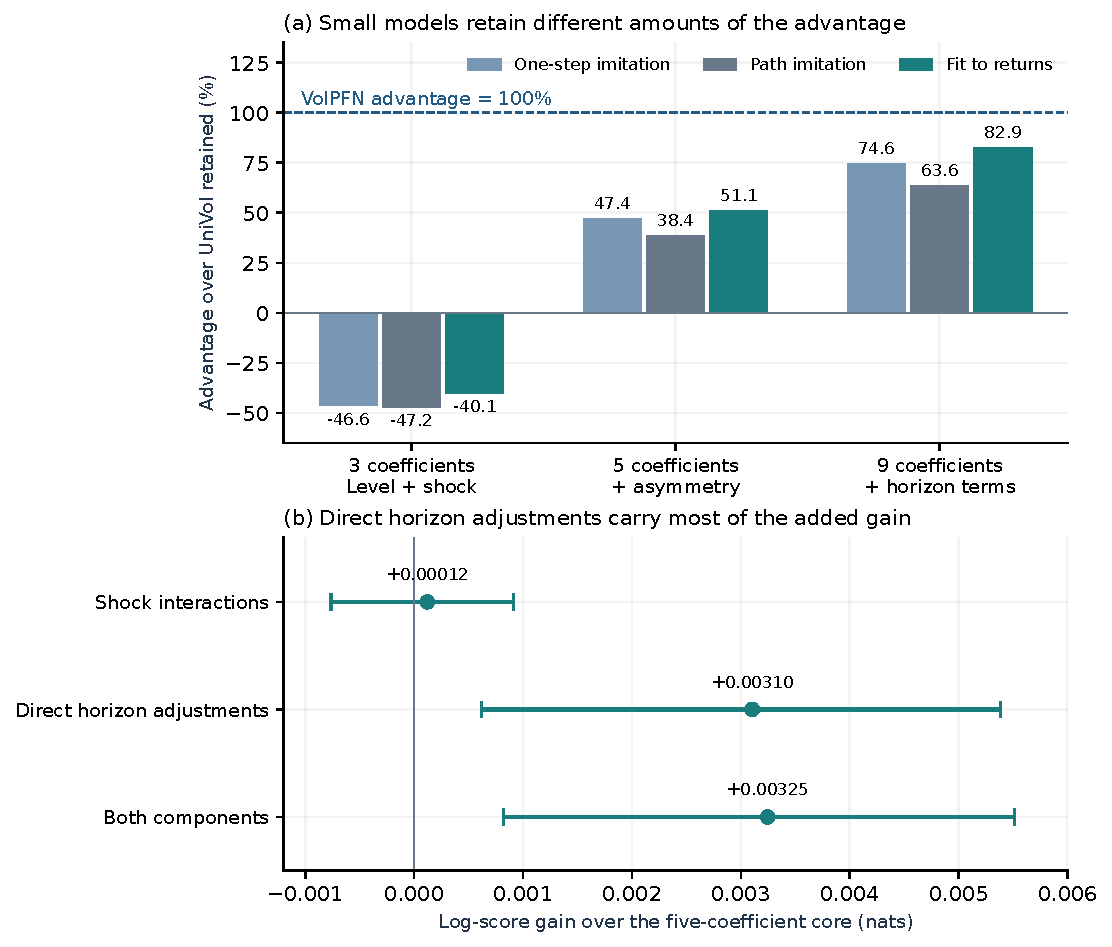
\includegraphics[width=\textwidth]{analysis_compact_rule.pdf}
\caption[Historical compact recovery and driver diagnostics]{Historical development evidence under common-$t_8$ scoring. Top: the original compression study's recovery fractions; 100\% is the retained network's advantage over UniVol, not perfect prediction. Bottom: the separate driver study's attained likelihood-fitted gains over the asymmetric core, with archived marginal 95\% calendar-block intervals. The driver alternatives have unequal optimisation success. Fitting to returns and imitating the network are different objectives; the two nine-coefficient results are separate fits.}
\label{fig:compact-components}
\end{figure}

A large network is therefore not the only way to retain much of this earlier checkpoint's scale performance. The compact evidence supports a predictive alternative while leaving internal computation and full-distribution recovery outside its claim.

\subsection{Supporting checks of objective and prior restriction}

Supporting STES comparisons show that the fitting loss can change the apparent usefulness of horizon inputs: STES changes the weight on recent observations as conditions change. Earlier smaller-network tests also favour completed broad-prior runs, but one broad seed fails, leaving only two genuine broad-versus-narrow pairs. Appendix~\ref{sec:supplementary-analysis} reports both. They motivate caution about objectives and diversity without replacing the five-pair experiment.

\section{Synthetic tracking as a limit on the explanation}

Synthetic tracking tests the stronger explanation that the network follows known variance changes nearly as well as a reference with extra information. Scoring against true simulated variance avoids squared-return proxy noise, although the input returns remain noisy. Up and down jumps have no artificial reflecting boundaries. The defective older lattice reference remains excluded.

Varying change frequency and sequence length gives 170 cells across five seeds. Comparators include compact rules, restarting predictors \citep{herbster1998tracking,hazan2009efficient}, a hindsight-selected filter and a known-model numerical reference. Market-fitted and separately simulation-fitted rules distinguish transfer difficulty from the predictive benefit of refitting the formula.

We exclude the first one hundred observations and compare each forecast with true simulated variance through expected QLIKE:

\begin{equation}
 \sum_{t\geq100}\left\{
 \frac{h_t^*}{\widehat h_t}-\log\!\left(\frac{h_t^*}{\widehat h_t}\right)-1\right\}.
 \label{eq:path-qlike-regret}
\end{equation}

True variance is $h_t^*$ and forecast variance is $\widehat h_t$. The loss compares these quantities directly because the simulation records the variance that generated each return. It thus tests tracking of the simulated state, whereas market QLIKE relies on an observed proxy. Summed path loss is divided by the realised jump count, or one when no jump occurs. This expresses error relative to changes in the tested setting without equalising detection difficulty or quiet-period forecasting cost across lengths.

The references are privileged. The numerical method knows the law and initial state and sets support from the realised path; the fixed filter is chosen with hindsight. Only seven of eighteen simulation-fitted explicit rules converge. These information and fitting differences define the test of the tracking explanation, rather than a comparison of architectures on equal opportunity (Appendix~\ref{sec:supplementary-analysis}).

\begin{table}[!htbp]
\centering
\caption[Synthetic variance-switching results]{Per-jump expected QLIKE loss in the sparse setting $\delta=2$, $V=8$. Each entry averages five paths. The selected lengths illustrate the change across the full prespecified range; smaller is better.}
\label{tab:switching-paths}
\small
\begin{tabular}{lrrr}
\toprule
Forecast & $T=512$ & $T=4{,}096$ & $T=32{,}768$ \\
\midrule
Known-model numerical reference & 15.90 & 18.54 & 26.46 \\
Hindsight fixed-filter selection & 19.15 & 43.57 & 142.38 \\
Restart experts & 22.44 & 31.39 & 52.40 \\
VolPFN & 24.30 & 35.01 & 92.30 \\
Nine-parameter rule, simulation fit & 28.31 & 51.12 & 323.81 \\
Nine-parameter rule, market coefficients & 71.19 & 224.98 & 1,287.94 \\
\bottomrule
\end{tabular}
\end{table}

VolPFN handles long paths better than the market-fitted compact rule, but fails the pre-specified near-reference thresholds. Worst within-window ratios exceed both sparse and dense limits, and the proposed beyond-window deterioration rule also fails. The earlier error-growth claim remains withdrawn: goodness-of-fit values for differently transformed responses cannot distinguish logarithmic from polynomial growth. Appendix~\ref{sec:prior-interpretation-details} records the thresholds and ratios.

\begin{figure}[!htbp]
\centering
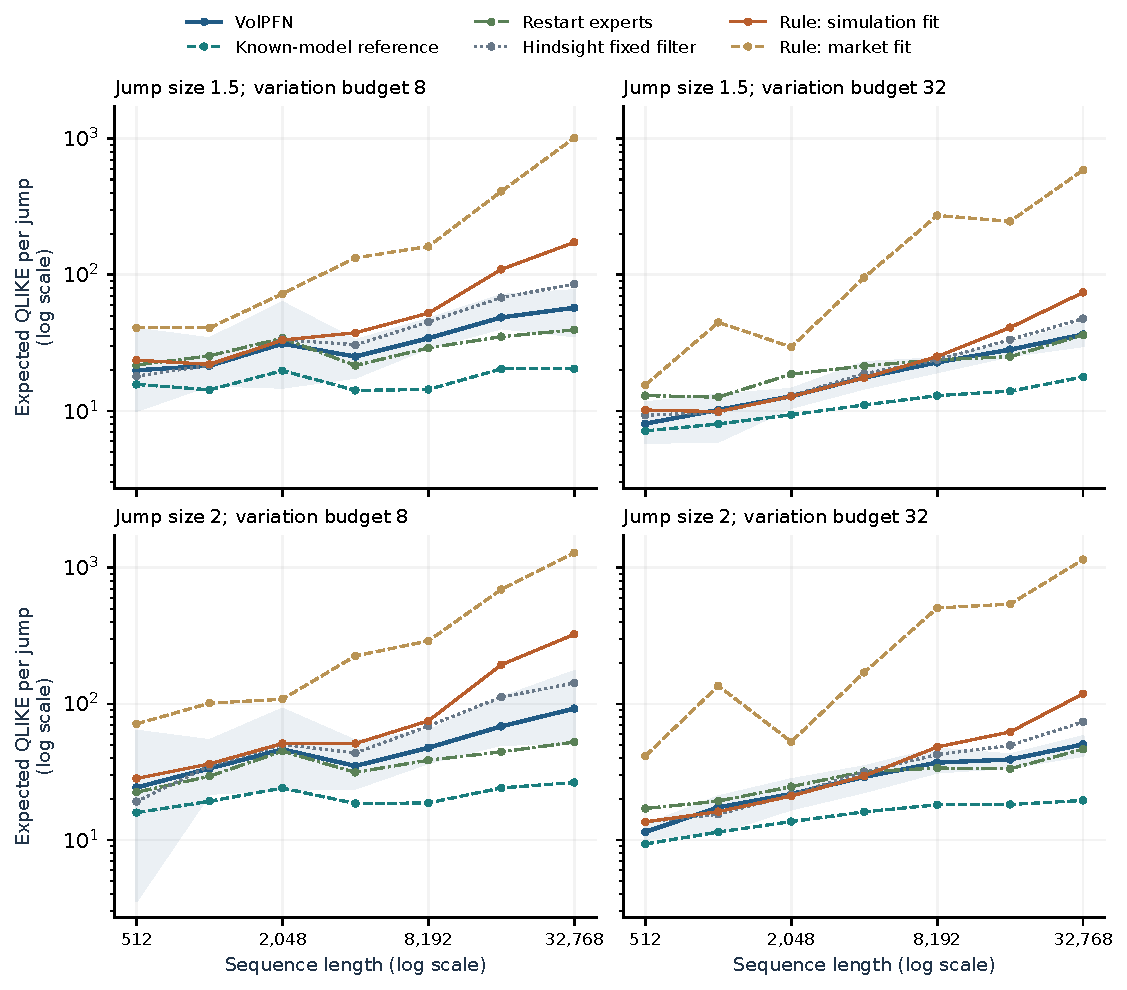
\includegraphics[width=\textwidth]{analysis_tracking_curves.pdf}
\caption[Tracking across the complete sparse sequence-length grid]{Mean per-jump expected QLIKE over five paths at every tested length in all four sparse settings. Lower is better; both axes use logarithmic spacing. The blue band spans the five observed VolPFN values, rather than a confidence interval. The known-model numerical reference and hindsight filter have additional information. The two compact-rule curves use nine coefficients fitted respectively on separate simulations and market data.}
\label{fig:tracking-curves}
\end{figure}

Figure~\ref{fig:tracking-curves} includes every tested sparse-grid length. Refitting improves the compact rule, but neither this nor the network's advantage establishes an asymptotic error rate. Some settings also depart from training in jump size or frequency. The results restrict the tracking explanation without invalidating the separate market comparisons.

The matched-prior gain and compact-rule recovery concern forecast scale. The failed tracking tests limit its proposed explanation. The next chapters examine the remaining prediction question: whether that scale assigns suitable probabilities to extreme losses.
